\subsubsection{\texttt{RF-10}: descarga de los ficheros de una propuesta propia de resolución de un ejercicio}
\label{subsec:rf10}

Dentro de la visualización del detalle de un curso matriculado, y tras escoger un directorio local para sincronizar los ficheros, un estudiante puede visualizar todos los ejercicios del curso diferenciados en distintos paneles según su estado de ejecución, tal como especifica el \referenciaConTT{subsec:rf9}{RF-9}.

En el caso de los ejercicios en progreso, al escoger el directorio, la aplicación buscará si existe una versión local del ejercicio, transitando entre los distintos estados reflejados en la \referenciaFigura{fig:reqf10-1}. En caso de no existir ninguna carpeta hija del directorio elegido coincidente con un ejercicio en progreso, la aplicación informará al usuario de que deberá descargar el punto de progreso que haya almacenado en el servidor, tal como ocurre con el ``Exercise 4'' en la \referenciaFigura{fig:reqf9-2}. Si, por el contrario, existe un directorio local que coincida con el ejercicio en progreso, la aplicación pregunta al usuario si desea descargar la versión existente en remoto y sobrescribir los ficheros que colapsen respecto a la versión en local o si, por el contrario, desea iniciar de inmediato la sincronización con el servidor. Este primer escenario es el que sucede en el caso del ``Exercise 1'' de la \referenciaFigura{fig:reqf9-2}.

Estos dos estados iniciales están reflejados en la parte izquierda de la \referenciaFigura{fig:reqf10-1}. Al descargar el ejercicio, se transita al estado que se observa en la parte central de la representación, durante el que la aplicación descarga como fichero comprimido los contenidos del ejercicio proporcionados por el servidor y los descomprime en una carpeta propicia específica dentro del directorio elegido por el estudiante, informando de forma visual a través de dos indicadores del estado activo y una barra de progreso. Una vez preparado el directorio del ejercicio, sea porque ha finalizado la descarga y descompresión o porque se ha iniciado la sincronización de contenidos previamente existentes, se inicia la sincronización automática, reflejada visualmente como muestra la parte derecha de la \referenciaFigura{fig:reqf10-1}. Esta sincronización queda detalladamente explicada en el requisito \referenciaConTT{subsec:rf11}{RF-11}.

\begin{figure}[ht]
    \centering
    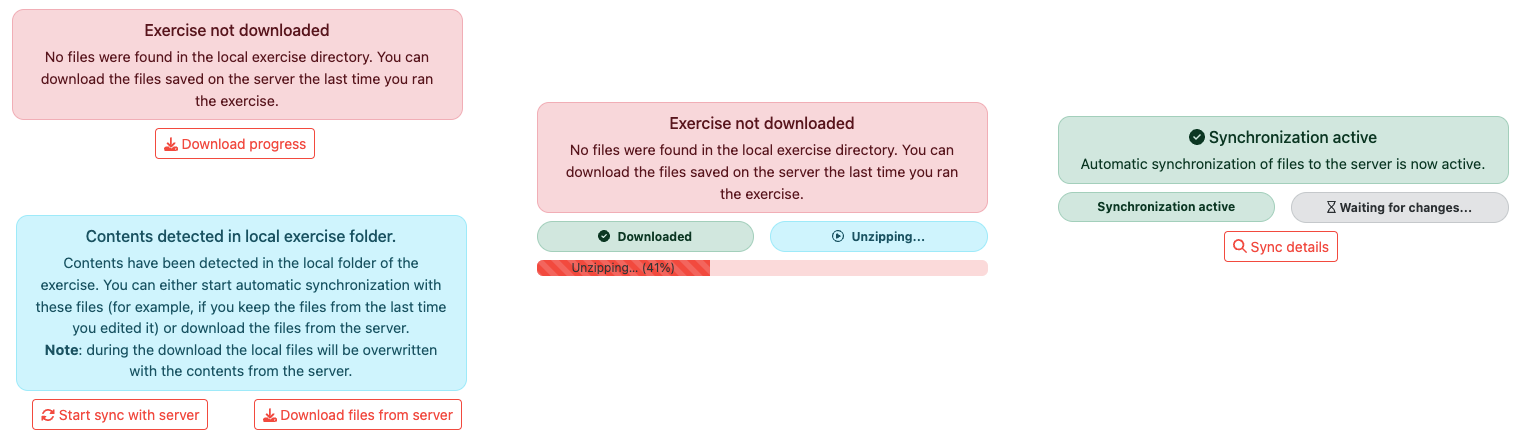
\includegraphics[width=\textwidth]{imagenes/utilizadas/4-3-implementacion/rf10-1.png}
    \caption{Representación de la evolución entre los posibles estados visuales de los ejercicios en progreso según su disponibilidad local.}
    \label{fig:reqf10-1}
\end{figure}
